% !TEX encoding   = UTF8
% !TEX root       = manual.tex
% !TEX spellcheck = en_US

\chapter{Going further: Editing tools}

When you have had some practise with {\Tw}, you'll find the need for more effective tools. Many of them are bundled with {\Tw}. We are going to see some of them now.

\section{Creating a document from a template}\index{template}

Most documents you will create will use the same instructions in the preamble, the same layout settings, similar heading and so on. You can use predefined templates to get started quickly or create your own with all of these settings already in place.

Use \menu{File}\submenu\menu{New from template\ldots} or \keysequence{Ctrl+Shift+N} (Mac OS X: \keysequence{Cmd+Shift+N}). A dialogue box opens to allow you to select one of the templates. After selecting one and pressing \verb|OK|, a document is created and you can start to work.

If you want to create a personal template, you just have to create a suitable document with everything you always want to do (and perhaps marking places to fill in the rest) and save it as a \path{.tex} file in the \path{<resources>\templates} folder, or a sub-folder of it, if you wish.

\section{Creating a project using several source files}\index{project}

When the source becomes long, it is sometimes difficult to navigate and maintain it. In that case, it is useful to split the source into different smaller files: one file will be the main document, with the preamble and the \verb|document| environment, as well as calls to the ``sub-documents''\footnote{Called by the commands
\verb|\input{}| or \verb|\include{}|, see {\LaTeX} manuals for more information.}, which could in turn contain separate chapters, for example.

But there might be a problem if you want to start typesetting/compilation in a sub-document: as there is neither a preamble nor a \verb|document| environment there, {\LaTeX} will stop immediately with an error.

To tell {\Tw} that it should typeset the main document, one adds at the very beginning of the sub-document the instruction:\index{\verb+% "!TeX+!\verb+root+}
\begin{verbExample}
% !TeX root = path/main_file.tex
\end{verbExample}
for example:
\begin{verbExample}
% !TeX root = manual.tex
\end{verbExample}

If the main file is in the same folder, its name is enough, as in the above example. Otherwise, you must also give the path to the main document (preferably relative to the sub-document in question, e.g., \path{../manual.tex}). Notice that the slash \verb|/| and not the backslash \verb|\| should be used as directory separator even on Windows.

Further, with MiKTeX, the call to a sub-document \verb|\input{name.tex}| should include the extension \path{.tex} to ensure proper SyncTeX functionality (see section~\ref{sec.synctex}).

\section{Spell-checking}

You can turn on automatic spell-checking\index{spell-checking} of your source document from \menu{Edit}\submenu\menu{Spelling}\submenu\menu{<language>}.

During typing, every word the spell-checker considers wrong is underlined by a red wavy line. A right-click on the word opens a contextual menu in which there are some replacement suggestions. Click on the desired word to make the replacement.

Before using the spell-checker, you need to install dictionaries in the right folder of {\Tw}: \path{<resources>\dictionaries}.

\begin{OSLinux}
On Linux, the dictionaries are usually taken from the folder \path{/usr/share/myspell/dicts}---the default path for myspell dictionaries. Note, though, that the maintainer of your {\Tw} package may have changed this to reflect the file system layout of your Linux distribution. You can override this default by setting the \verb+TW_DICPATH+ environment variable before running {\Tw}.
\end{OSLinux}

One can use the available dictionaries for OpenOffice.org and other free software;\footnote{See, for example, \url{http://lingucomponent.openoffice.org/download_dictionary.html}.} if you have Mozilla Thunderbird with spell-checking, you can copy its \path{.aff} and \path{.dic} files\index{spell-checking!.aff files}\index{spell-checking!.dic files} as well, for example. It is possible to ask {\Tw} to enable spell-checking by default by setting a dictionary in \menu{Edit}\submenu\menu{Preferences\dots}\submenu\menu{Editor}\submenu\menu{Spell-check language}.

\section{Search and replace}
\index{editing!search/replace}\index{search/replace|see {editing}}

\subsection{Standard functions}

The options of the menu \menu{Search}---\menu{Find\dots}, \menu{Find again}, \menu{Replace\dots}, \menu{Replace again}, and \menu{Go to Line\dots} (\keysequence{Ctrl+F}, \keysequence{Ctrl+G}, \keysequence{Ctrl+R}, \keysequence{Ctrl+Shift+R}, and \keysequence{Ctrl+L}, respectively)---are standard actions (Mac OS X: \keysequence{Cmd+F}, \keysequence{Cmd+G}, \keysequence{Cmd+R}, \keysequence{Cmd+Shift+R}, and \keysequence{Cmd+L}); the first and the third open a dialogue box:

\begin{center}
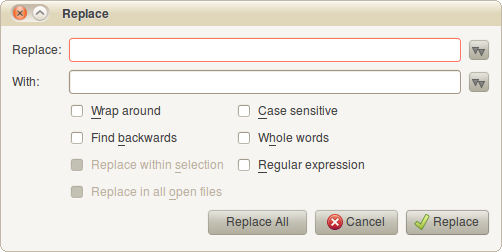
\includegraphics[scale=.6]{replaceDialog}
\end{center}

Here, the usual options are available: \emph{Wrap around}, \emph{Find backwards}, \emph{Search/Replace within selection}, or \emph{Find all occurrences}. The following options are also usual: \emph{Case sensitive} and \emph{Whole words}. By default, the search is forward, towards the end of the document.

The option \emph{Search/Replace in all open files} is also a frequent choice, but not as much as the others; this allows, for example, replacement in all the files of a project---pay attention, though, as this is very powerful.

The last option, \emph{Regular expression}, is detailed in the next sub-section.

In the \menu{Search} menu there are other options:
\begin{description}
\item[Copy to Find] copies the currently selected text into the \textsl{\textbf{Find}} field of the Find dialogue or the \textsl{\textbf{Replace}} field of the Replace dialogue; you still need to open the dialogues separately
\item[Copy to Replace] copies the currently selected text into the \textsl{\textbf{With}} field of the \textsl{\textbf{Replace}} dialogue
\item[Find Selection] uses the current selection for a search without opening the \textsl{\textbf{Find}} dialogue---very fast
\item[Show selection] scrolls the view to the currently selected text---useful if word wrapping is turned off and you moved in the document using the vertical scroll bar on the right
\end{description}

\subsection{Advanced search and replace (regular expressions)}\index{regular expressions}

The regular expressions provide a very powerful tool, but they require some effort to be well understood. To understand them fully would require a manual of its own\footnote{Such manuals exist on the internet.}, so we'll only give some simple ideas of use. For more advanced uses, as well as lists of the most used codes, see section \ref{sec:regexp}.

Suppose we have the following text:
\begin{verbExample}
Voici du texte pour tester les expressions régulières dans du texte
accentué. 
Voici du texte pour tester les expressions régulières dans du texte
accentué. 
Voici du texte pour tester les expressions régulières. Voici du
texte pour tester les expressions régulières. 
truc          truc
tél.: 010-99-99-99
tél.: 00.32.10.99.99.99
tél.: 00/32-10/99.99.99
\end{verbExample}
We want to
\begin{enumerate}
	\item insert an empty line after each ``accentué'' (to create paragraphs in {\LaTeX}), but not after the three telephone numbers;
	\item replace each \textsl{tab} character between the two words ``truc'' of the fourth paragraph by three spaces; and finally
	\item make the telephone numbers consistent by replacing the various punctuation characters by spaces.
\end{enumerate}

For 1., in the dialogue box \textsl{\textbf{Replace}} (\keysequence{Ctrl+R}) for \emph{Replace:} we put {\frq\verb+\n+\flq}\footnote{the {\frq\flq} are used here only to show the limits of the entered text and they should not actually be entered.} and in \emph{With:} {\frq\verb+\n\n+\flq}. {\frq\verb+\n+\flq} is the code to match or insert a line feed. You will need to select the first four paragraphs and the beginning of the fifth (the first telephone number) and to tick the \emph{Replace within selection} and \emph{Regular expression} options; if this was not done and an empty line has been inserted after each line, select the telephone lines and do the reverse action: replace {\frq\verb+\n\n+\flq} by {\frq\verb+\n+\flq}. So we replaced one line feed by two, creating an empty line.

For 2., use {\frq\verb+\t+\flq} and {\frq\verb*+   +\flq}\footnote{These are three space characters.}. {\frq\verb+\t+\flq} is the code which represents a tab, while a space is typed in literally (here represented as \verb*| |).

For 3., find {\frq\verb+-|\.|/+\flq} and replace with {\frq\verb*+ +\flq}. Here, {\frq\verb+|+\flq} provides alternatives (\verb|-|, \verb|.|, or \verb|/|); for the dot we have used {\frq\verb+\.+\flq} because the dot alone is a regular expression code which represents any character and we would have replaced all the characters by spaces! We therefore have to use a code---prefixing the dot with a backslash tells specifies that the normal meaning of the dot should be used instead of the special meaning it usually has in regular expressions.

If one has strings of the same character but of different lengths (for example 3, 4, or 5 times the sames character e) and one wants to truncate all these strings to a string with less characters (for example 2), one can ask to replace the string {\frq\verb+e{3,5}+\flq} by {\frq\verb+ee+\flq}.

If one wants to insert the same string at the beginning of some paragraphs separated or not by an empty line, for example {\frq\verb*+\noindent +\flq} or {\frq\verb*+\item +\flq}, one can replace {\frq\verb+\n\n+\flq} or {\frq\verb+\n+\flq} by {\frq\verb*+\n\n\\noindent +\flq} or {\frq\verb*+\n\\noindent +\flq}. Pay attention, we have a double \verb|\| in front of \verb|noindent| to get one (\verb|\noindent|) because \verb|\| is an escape character in regular expressions (we've met it before in the expression \verb|\.|)!

If it were making sense, we could replace all the letters between ``a'' and ``m'' by ``\$'' using {\frq\verb+[a-m]+\flq} and {\frq\verb+$+\flq}.

\section{Other tools for editing and error tracking\index{editing!tools}}

\subsection{Standard tools}

It is always possible to undo\index{editing!undo} an action using \menu{Edit}\submenu\menu{Undo} or \keysequence{Ctrl+Z} (Mac OS X: \keysequence{Cmd+Z}): this way you can undo stepwise! The inverse action, redo, is available as \menu{Edit}\submenu\menu{Redo}\index{editing!redo} or \keysequence{Ctrl+Shift+Z} (Mac OS X: \keysequence{Cmd+Shift+Z}).\footnote{\keysequence{Ctrl+Y} and \keysequence{Alt+Shift+Backspace} work as well on Windows. \keysequence{Cmd+Y} work as well on Mac OS X.}

{\Tw} also provides the standard editing tools such as the clipboard; therefore one can select, cut/copy and paste a piece of text normally.

You can select with the mouse by dragging over the desired text, or by  double-clicking to select a word. Using the keyboard, holding down \keysequence{Shift} while moving using the arrow keys will select text. You can also move and select word by word moving left or right holding \keysequence{Ctrl+Shift} down (\keysequence{Cmd+Shift} on Mac OS X). The clipboard shortcuts are the ones you'll find in almost every program: \keysequence{Ctrl+X} to cut, \keysequence{Ctrl+C} to copy, and \keysequence{Ctrl+V} to paste (\keysequence{Cmd+X}, \keysequence{Cmd+C} and \keysequence{Cmd+V}, respectively, on Mac OS X).

You can easily change the case\index{editing!change case} of a selection---put everything upper case or lower case---using \menu{Edit}\submenu\menu{Change case} and next, depending on the desired effect, \menu{ALL UPPERCASE}, \menu{all lowercase}, or \menu{Toggle Case} (which toggles the case of each letter individually).

It is also convenient to show the line numbers\index{editing!line numbers}, as all error messages refer to these numbers; you can toggle the line numbers, on the left of the editing panel, from \menu{Format}\submenu\menu{Line Numbers}.

\subsection{Commenting}

When preparing a document with {\AllTeX}, it is often useful to prevent compilation of a portion of text to be able to locate an error; you can do this piece by piece until you find the part which causes the error. For that, commenting the source block by block is needed. 

We have seen that the symbol \verb+%+ marks the beginning of a comment.
To comment\index{editing!comment} a big piece of text, it is sufficient to select it and ask to mark it as comment \menu{Format}\submenu\menu{Comment} or \keysequence{Ctrl+Shift+]} (Mac OS X: \keysequence{Cmd+Shift+]}). To remove the comment, select the lines and choose \menu{Format}\submenu\menu{Uncomment}\index{editing!uncomment} or \keysequence{Ctrl+Shift+[} (Mac OS X: \keysequence{Cmd+Shift+[}).\footnote{On some keyboards, like the French one, it is impossible to use \keysequence{Ctrl+Shift+[} or \keysequence{Ctrl+Shift+]}; these shortcuts can be changed, however---see section \ref{sec.shortcuts}}

\subsection{Matching delimiters}

A frequent error is to forget a closing symbol: parenthesis, bracket, square bracket, \emph{etc}. {\Tw} helps with a tool to show the pairs of symbols: when the cursor moves over one of these symbols, its partner is briefly highlighted. You can also select an entire block\index{editing!select a block} using \menu{Edit}\submenu\menu{Balance Delimiters} or by the shortcut \keysequence{Ctrl+B} (Mac OS X: \keysequence{Cmd+B}). Thus, you will immediately see the scope of the block.

\subsection{Smart quotes}

Another similar error, but this time semantic and not hindering typesetting, is in the use of quotes when one wants to give focus to some text.

There are two types of quotation marks in English: the `single' quotes and the ``double'' quotes. They are formed by ` and '; these are not the quotation marks used in programming and found on the keyboard: \verb|"| and \verb|'|. Using the {\Tw} smart quotes system, one can use the latter as normal to automatically produce the typographically correct single/double opening and close quotes.

In a \path{.tex} document, select one of the smart quotes system: \menu{Format}\submenu\menu{Smart Quotes}\submenu\menu{TeX Ligatures}, \submenu\menu{TeX Commands}, \submenu\menu{Unicode Characters}. Then, when you want to start a quoted section in your text, let's say enclosed in double quotes, type \verb|"|, then the text to be quoted, and finish again by \verb|"|; {\Tw} will automatically insert the correct opening quotes \verb|``| and later the correct closing ones \verb|''|. The three options give the same result in the typeset document, but \menu{TeX Ligatures} should work best in most cases.

Finally, it is possible to define personal quotation marks systems (in the file \path{smart-quotes-modes.txt} in the \path{configuration} folder of the resource folder).

\section{Auto-completion\index{auto-completion}}

Another tool which rapidly becomes indispensable is auto-completion. Indeed, when you use {\AllTeX}, you have to continuously enter codes to, for example, create environments; you also have to remember to close every group you open.

Auto-completion allows you to type a keyword, hit the \keysequence{Tab} key, and have {\Tw} insert the {\AllTeX} command or environment code automatically.

As an example to insert ``\LaTeX'', we have to type \verb|\LaTeX|. This is not difficult, but entering ``\verb|\|'' followed by the word ``\verb|LaTeX|'' with alternating capitals and lower case letters could become annoying after a while.\footnote{In particular with keyboard layouts where \texttt{\textbackslash} is not directly accessible.} With auto-completion, you just enter \verb|latex| and hit \keysequence{Tab} to get \verb|\LaTeX|. You just have to take care that there is no \emph{letter} directly preceding or succeeding \verb|latex|---e.g., \verb|alatex|---, or else the mechanism might not pick up the correct keyword.

\needspace{3\baselineskip}
Another example is \verb|bmin|, which gives
\begin{verbExample}
\begin{minipage}{}
•
\end{minipage}•
\end{verbExample}
with the cursor between the empty pair of curly brackets where you need to enter the size of the minipage. See the section \ref{sec.autocompletion} for a list of the keywords for auto-completion. Notice the ``•'' in the minipage environment. They are placeholders which can be reached by \keysequence{Ctrl+Tab} (\keysequence{Opt+Tab} on the Mac), repeating this shortcut cycles forward through the placeholders; by \keysequence{Ctrl+Shift+Tab} (\keysequence{Opt+Shift+Tab}), you can also cycle backwards.

If a partial keyword is given, repeatedly hitting \keysequence{Tab} will cycle through possible completions. For example, \verb|bali| (the \verb|b| commonly indicates the beginning of an environment, \verb|\begin{}|) creates the \verb|align| environment after one \keysequence{Tab}, next \verb|align*|, and after that, in succession, \verb|alignat|, \verb|alignat*|, \verb|aligned|, \verb|alignedat|, and \verb|alignedat| with options; to access the last environments directly, they have their own codes which start by \verb|bali| (\verb|balis|, \verb|baliat|, \verb|baliats|, \verb|balied|, \verb|baliedat| and \verb|baliedato|).

If you want to create your own keywords, you can add a \path{.txt} file in the \path{completion} folder inside the resources folder. The entries in the file should have the following format:
\begin{verbExample}
bfigo:=\begin{figure}[#INS#]#RET##RET#\end{figure}•
\bibliography{#INS#}•
\end{verbExample}

In the first case, \verb|bfigo| is the assigned keyword (with \verb|:=|) to be converted into a \verb|figure| environment with an optional argument; there are two carriage returns (\verb|#RET#|) after the \verb|begin|, i.e., an empty line, and the cursor is placed between the square brackets (at the position of \verb|#INS#|). ``•'' is a place holder as introduced before.

In the second case, we give ourselves a shortcut, which will let us type the first part of \verb|\bibliography{}| and have {\Tw} convert it to the full name plus braces (with the cursor between them). In this case, the keyword is the instruction itself.

Note that the \path{.txt} file containing the auto-completion information needs to be UTF-8 encoded---this is the default encoding for all files created with {\Tw}.